% Customizable fields and text areas start with % >> below.
% Lines starting with the comment character (%) are normally removed before release outside the collaboration, but not those comments ending lines

% svn info. These are modified by svn at checkout time.
% The last version of these macros found before the maketitle will be the one on the front page,
% so only the main file is tracked.
% Do not edit by hand!
\RCS$Revision: 401991 $
\RCS$HeadURL: svn+ssh://svn.cern.ch/reps/tdr2/notes/HIG-17-005/trunk/HIG-17-005.tex $
\RCS$Id: HIG-17-005.tex 401991 2017-05-02 11:20:47Z stiegerb $
%%%%%%%%%%%%% local definitions %%%%%%%%%%%%%%%%%%%%%
% This allows for switching between one column and two column (cms@external) layouts
% The widths should  be modified for your particular figures. You'll need additional copies if you have more than one standard figure size.
\newlength\cmsFigWidth
\ifthenelse{\boolean{cms@external}}{\setlength\cmsFigWidth{0.85\columnwidth}}{\setlength\cmsFigWidth{0.4\textwidth}}
\ifthenelse{\boolean{cms@external}}{\providecommand{\cmsLeft}{top\xspace}}{\providecommand{\cmsLeft}{left\xspace}}
\ifthenelse{\boolean{cms@external}}{\providecommand{\cmsRight}{bottom\xspace}}{\providecommand{\cmsRight}{right\xspace}}
%%%%%%%%%%%%%%%  Title page %%%%%%%%%%%%%%%%%%%%%%%%
\cmsNoteHeader{HIG-17-005} % This is over-written in the CMS environment: useful as preprint no. for export versions
\newcommand{\GeVnn}{\ensuremath{{\,\text{Ge\hspace{-.08em}V\hspace{-0.16em}}}}\xspace}
\newcommand{\CLs}{CL\ensuremath{_\mathrm{S}}\xspace}
% >> Title: please make sure that the non-TeX equivalent is in PDFTitle below
\title{Search for production of a Higgs boson and a single top quark in
multilepton final states in proton collisions at $\sqrt{s}=13$~TeV}

\def    \pt         {\mbox{$p_{\mathrm{T}}$}\xspace}
\def    \mt         {\mbox{$m_{\mathrm{T}}$}}
\def    \mgg        {\mbox{$m_{\gamma\gamma}$}}
\def    \mll        {\mbox{$m_{\ell\ell}$}}
\def    \mh         {\mbox{$m_{\mathrm{H}}$}}
\def    \tth        {\mbox{$\mathrm{t}\bar{\mathrm{t}}\mathrm{H}$}}
\def    \thq        {\mbox{$\mathrm{tHq}$}}
\def    \ttgg       {\mbox{$\mathrm{t}\bar{\mathrm{t}}\gamma\gamma$}}
\def    \ttg        {\mbox{$\mathrm{t}\bar{\mathrm{t}}\gamma$}}
\def    \tgg        {\mbox{$\mathrm{t}\gamma\gamma$}}
\def    \hgg        {\mbox{$\mathrm{H}\rightarrow\gamma\gamma$}}
\def    \met        {\mbox{$E_\mathrm{T}^\mathrm{miss}$}}
\def    \lumi       {\mbox{$L = 19.7$~\fbinv}}

\newcommand{\W}{\ensuremath{\cmsSymbolFace{W}}\xspace}
\newcommand{\ZZ}{\ensuremath{\cmsSymbolFace{ZZ}}\xspace}
\newcommand{\WW}{\ensuremath{\cmsSymbolFace{WW}}\xspace}
\newcommand{\WZ}{\ensuremath{\cmsSymbolFace{WZ}}\xspace}
\newcommand{\VVV}{\ensuremath{\cmsSymbolFace{VVV}}\xspace}
\newcommand{\WVV}{\ensuremath{\cmsSymbolFace{WVV}}\xspace}
\newcommand{\tautau}{\ensuremath{\Pgt\Pgt}\xspace}
\newcommand{\gaga}{\ensuremath{\Pgg\Pgg}\xspace}
\newcommand{\ttW}{\ensuremath{\ttbar\cmsSymbolFace{W}^{\pm}}\xspace}
\newcommand{\ttWW}{\ensuremath{\ttbar\WW}\xspace}
\newcommand{\ttZ}{\ensuremath{\ttbar\cmsSymbolFace{Z}}\xspace}
\newcommand{\ttH}{\ensuremath{\ttbar\cmsSymbolFace{H}}\xspace}
\newcommand{\ttG}{\ensuremath{\ttbar\gamma}\xspace}
\newcommand{\ttV}{\ensuremath{\ttbar\cmsSymbolFace{V}}\xspace}
\newcommand{\ttGStar}{\ensuremath{\ttbar\gamma^*}\xspace}
\newcommand{\tZq}{\ensuremath{\cPqt\Z\Pq}\xspace}

%\newcommand{\WWqq}{\ensuremath{\PWp\PWp{\rm qq}}\xspace}
%\newcommand{\WWDPI}{\ensuremath{\PWp\PWp(\mathrm{DPI})}\xspace}

\newcommand{\WWqq}{\ensuremath{\W^{\pm}\W^{\pm}{\rm qq}}\xspace}
\newcommand{\WWDPI}{\ensuremath{\W^{\pm}\W^{\pm}(\mathrm{DPI})}\xspace}

\newcommand{\epem}{\ensuremath{\cmsSymbolFace{e^+e^-}}\xspace}
\newcommand{\udsgjet}{\ensuremath{\cPqu\cPqd\cPqs\cPg\text{-jet}}\xspace}
\newcommand{\cjet}{\ensuremath{\cPqc\text{-jet}}\xspace}
\newcommand{\bjet}{\ensuremath{\cPqb\text{-jet}}\xspace}
\newcommand{\bjets}{\ensuremath{\cPqb\text{-jets}}\xspace}
\newcommand{\CV}{\ensuremath{\kappa_\text{V}}\xspace}
\newcommand{\Ct}{\ensuremath{\kappa_\cPqt}\xspace}

% Macros for THq:
\newcommand{\Hbb}{\ensuremath{\PH\rightarrow\rm{b\overline{b}}}\xspace}
%\newcommand{\HWW}{\ensuremath{\PH\rightarrow\PWp\PWm}\xspace}
\newcommand{\HWW}{\ensuremath{\PH\rightarrow\W\W}\xspace}
\newcommand{\HZZ}{\ensuremath{\PH\rightarrow\Z\Z}\xspace}
\newcommand{\HTT}{\ensuremath{\PH\rightarrow\tautau}\xspace}
\newcommand{\Htautau}{\ensuremath{\PH\rightarrow\tautau}\xspace}
\newcommand{\Hgg}{\ensuremath{\PH\rightarrow\gaga}\xspace}
\newcommand{\tHqWW}{\ensuremath{\cPqt\PH(\W\W)\mathrm{q}}\xspace}
\newcommand{\tHqtt}{\ensuremath{\cPqt\PH(\tautau)\mathrm{q}}\xspace}
\newcommand{\tHWWW}{\ensuremath{\cPqt\PH(\W\W)\W}\xspace}
\newcommand{\tHWtt}{\ensuremath{\cPqt\PH(\tautau)\W}\xspace}
\newcommand{\tHq}{\ensuremath{\cPqt\PH\mathrm{q}}\xspace}
\newcommand{\tHW}{\ensuremath{\cPqt\PH\W}\xspace}
\newcommand{\tH}{\ensuremath{\cPqt\PH}\xspace}

% Channels
\newcommand{\ee}{\ensuremath{\Pe\Pe}\xspace}
\newcommand{\emu}{\ensuremath{\Pe\Pgm}\xspace}
\newcommand{\mumu}{\ensuremath{\Pgm\Pgm}\xspace}
\newcommand{\threel}{\ensuremath{\ell\ell\ell}\xspace}

% >> Authors
%Author is always "The CMS Collaboration" for PAS and papers, so author, etc, below will be ignored in those cases
%For multiple affiliations, create an address entry for the combination
%To mark authors as primary, use the \author* form
%\address[neu]{Northeastern University}
%\address[fnal]{Fermilab}
%\address[cern]{CERN}
%\author[cern]{The CMS Collaboration}

% >> Date
% The date is in yyyy/mm/dd format. Today has been
% redefined to match, but if the date needs to be fixed, please write it in this fashion.
% For papers and PAS, \today is taken as the date the head file (this one) was last modified according to svn: see the RCS Id string above.
% For the final version it is best to "touch" the head file to make sure it has the latest date.
\date{\today}

% >> Abstract
% Abstract processing:
% 1. **DO NOT use \include or \input** to include the abstract: our abstract extractor will not search through other files than this one.
% 2. **DO NOT use %**                  to comment out sections of the abstract: the extractor will still grab those lines (and they won't be comments any longer!).
% 3. For PASs: **DO NOT use tex macros**         in the abstract: CDS MathJax processor used on the abstract doesn't understand them _and_ will only look within $$. The abstracts for papers are hand formatted so macros are okay.
\abstract{Additional material for HIG-17-005}

% >> PDF Metadata
% Do not comment out the following hypersetup lines (metadata). They will disappear in NODRAFT mode and are needed by CDS.
% Also: make sure that the values of the metadata items are sensible and are in plain text:
% (1) no TeX! -- for \sqrt{s} use sqrt(s) -- this will show with extra quote marks in the draft version but is okay).
% (2) no %.
% (3) No curly braces {}.
\hypersetup{%
pdfauthor={Jose Monroy, Benjamin Stieger, Pallabi Das, Sandhya Jain},%
pdftitle={Additional material for HIG-17-005},%
pdfsubject={CMS},%
pdfkeywords={CMS, physics, higgs, top, tHq, multilepton}}

\maketitle

\begin{figure}[!htb]
  \begin{center}
    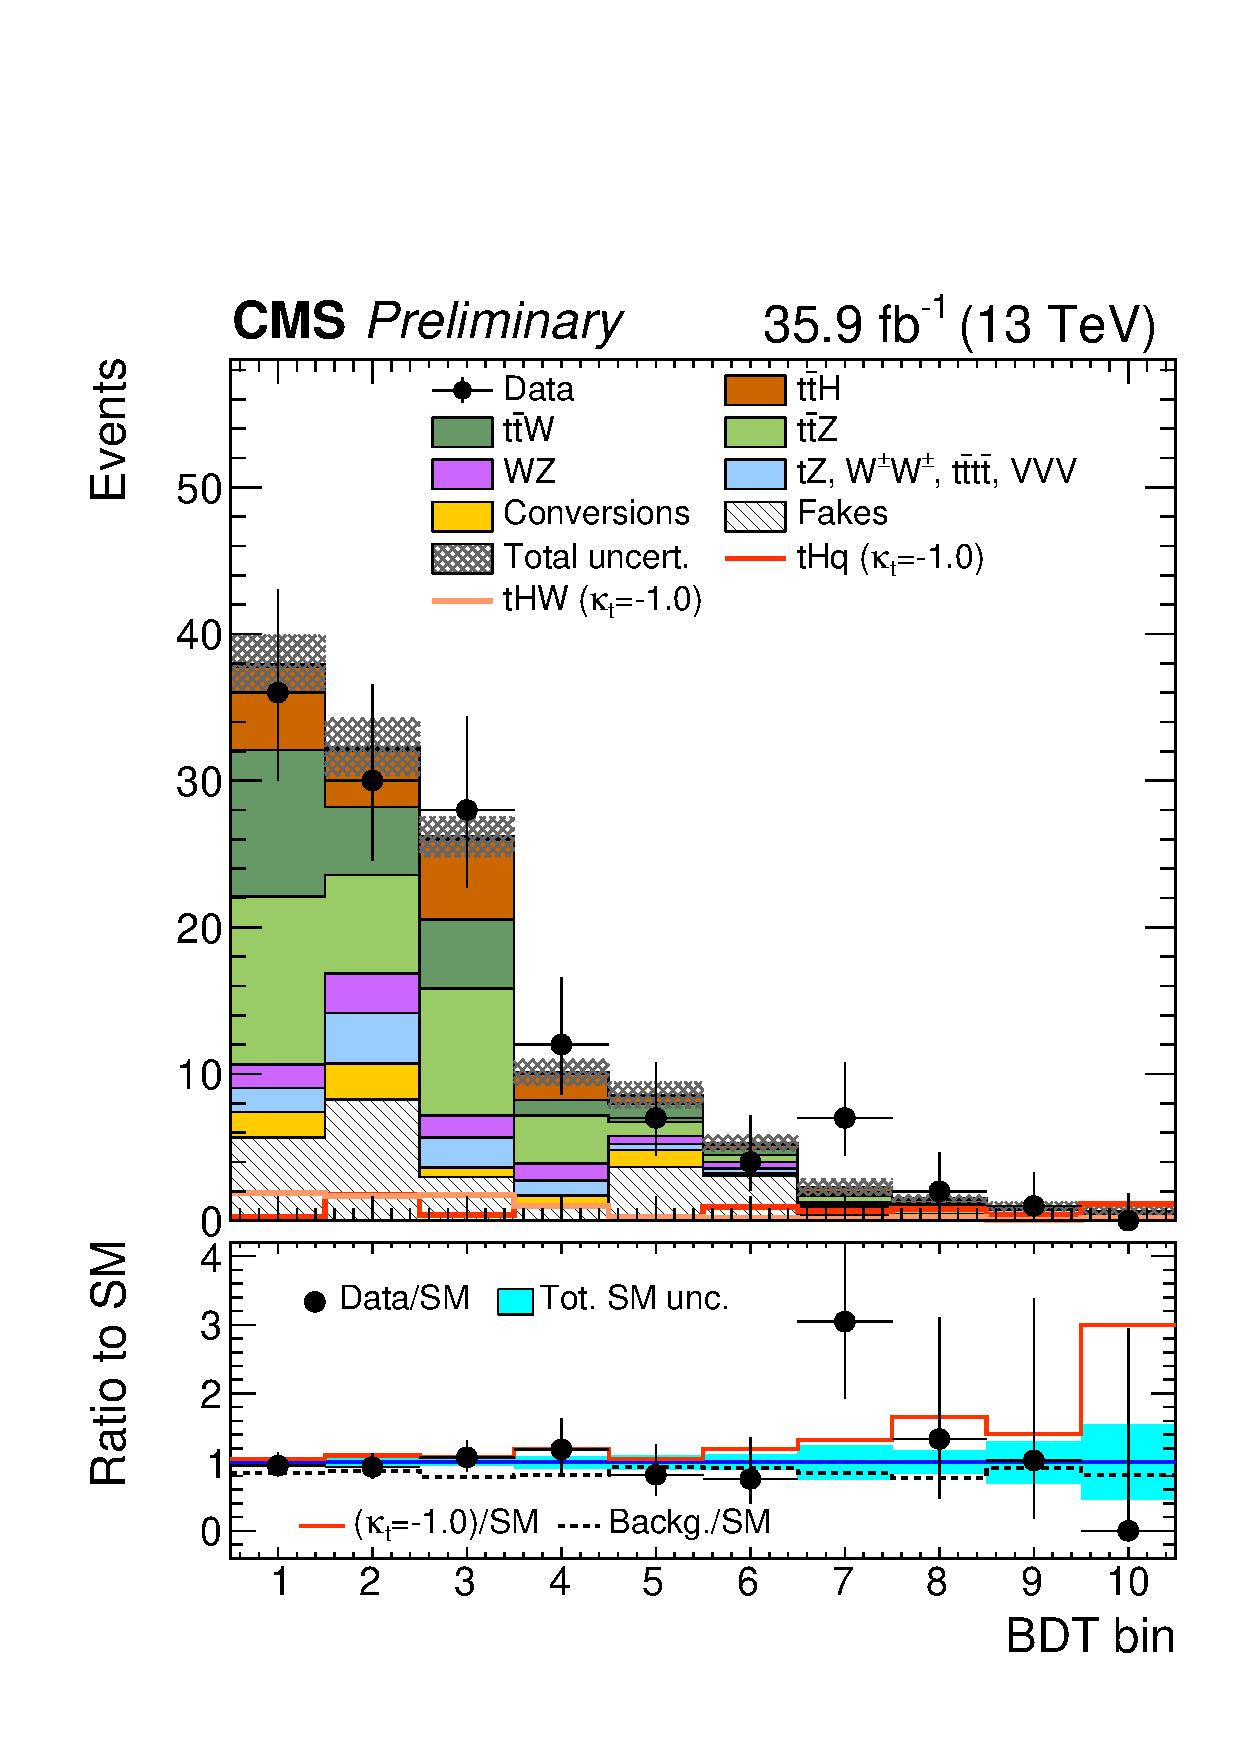
\includegraphics[width=0.32\textwidth]{Figures/polished/finalBins_40_3l.pdf}
    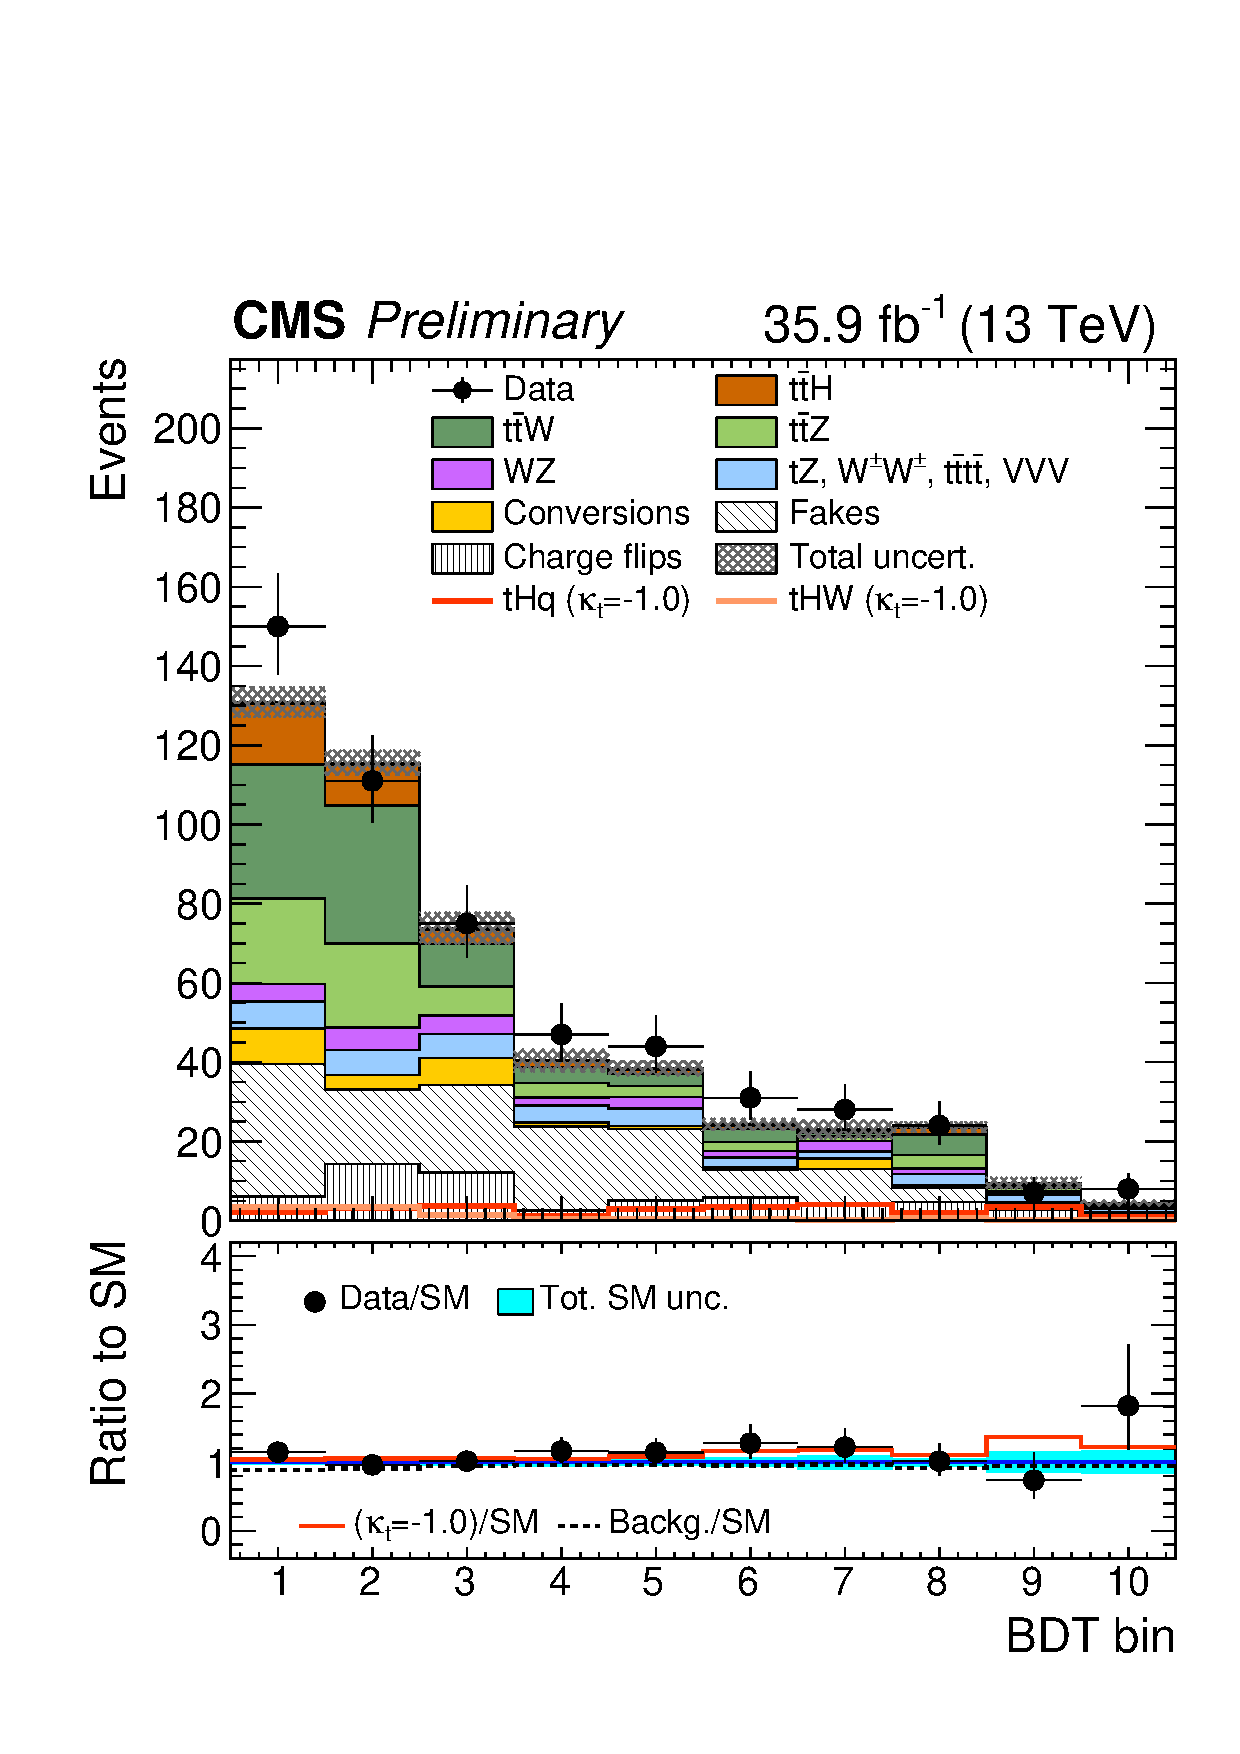
\includegraphics[width=0.32\textwidth]{Figures/polished/finalBins_40_em.pdf}
    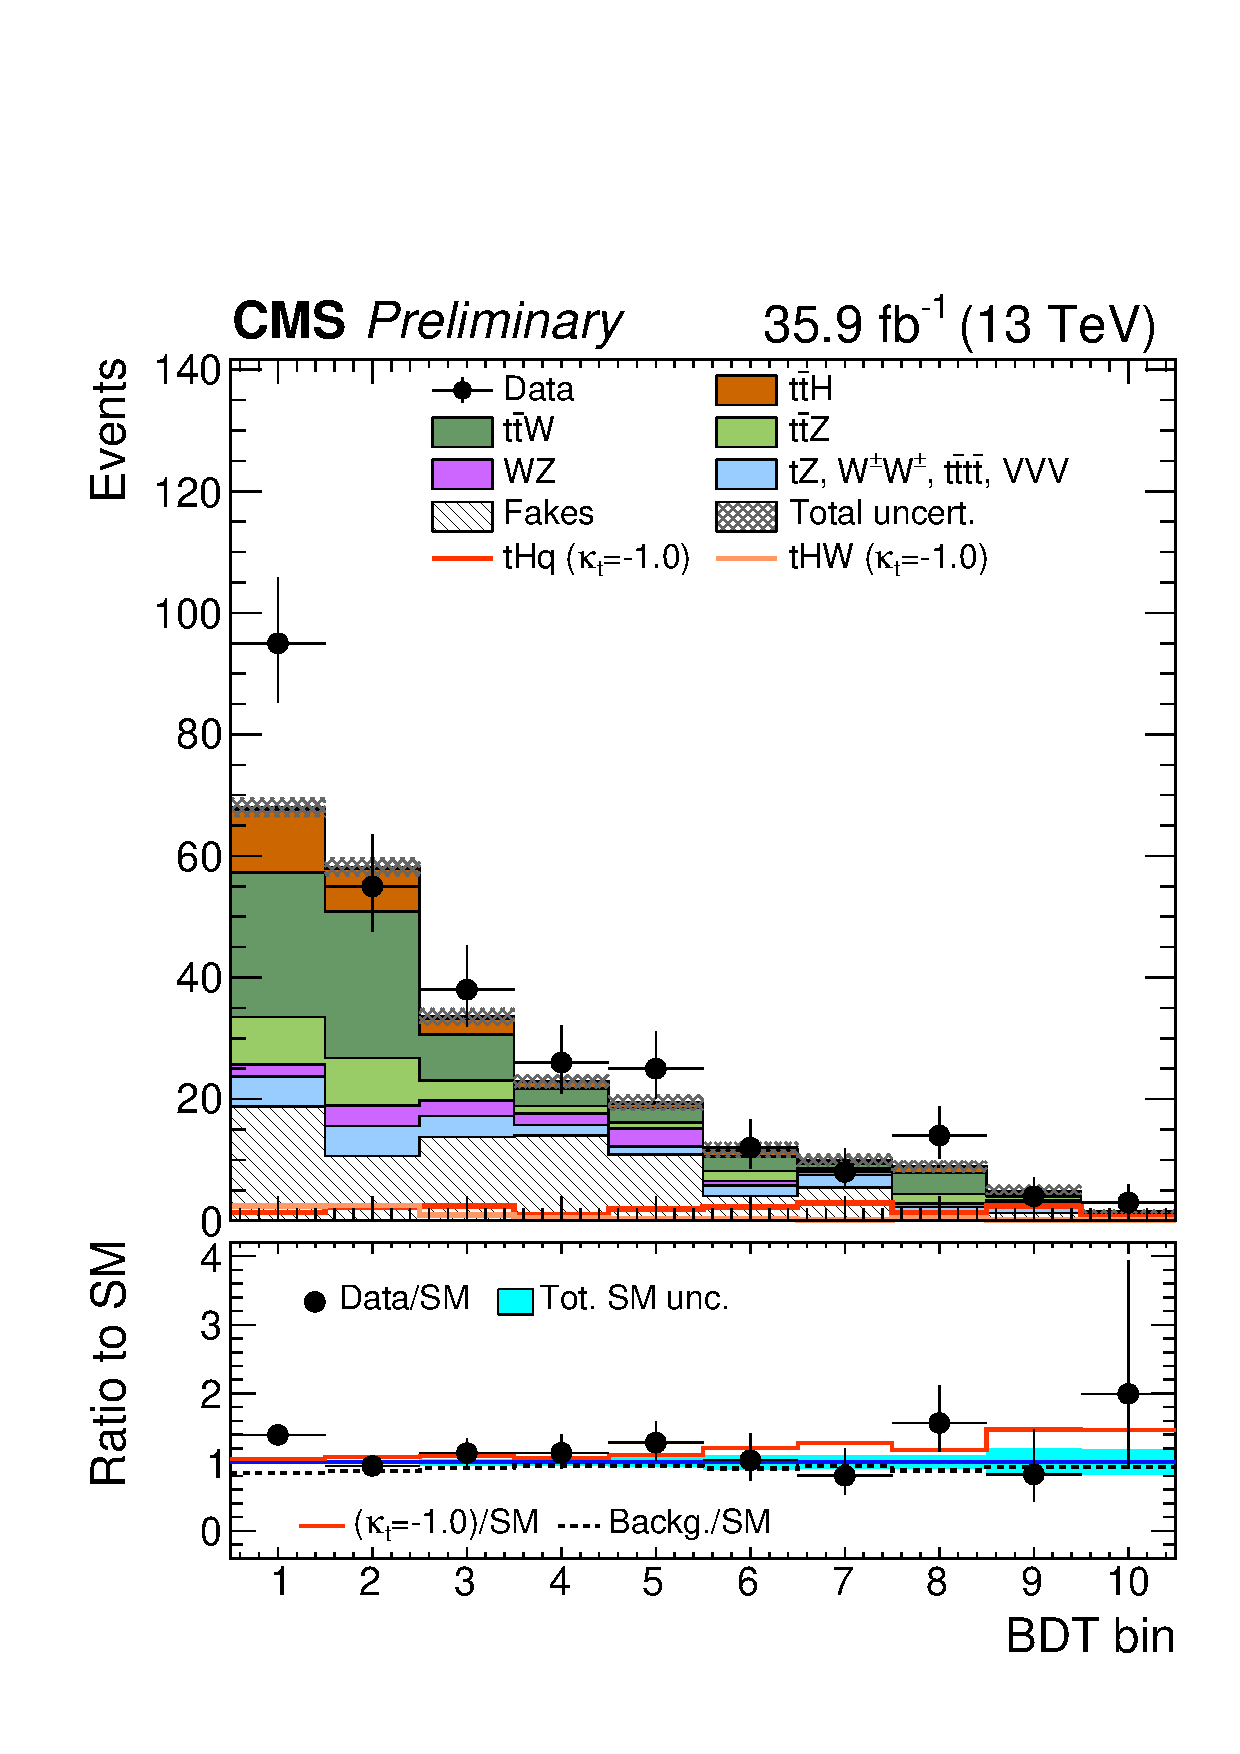
\includegraphics[width=0.32\textwidth]{Figures/polished/finalBins_40_mm.pdf}
  \end{center}
  \caption{Pre-fit categorized BDT classifier outputs, for the three-lepton channel (left), \emu\ (center), and \mumu\ (right), for 35.9~\fbinv.
  In the box below each distribution, the ratio of the observed and predicted event yields is shown.
  The shape of the two \tH\ signals for $\Ct=-1.0$ is shown, normalized to their respective cross sections for $\Ct=-1.0, \CV=1.0$.
  The grey band represents the unconstrained (pre-fit) statistical and systematical uncertainties.\label{fig:aux_prefit_finalbins}}
\end{figure}

\begin{figure}[!htb]
  \begin{center}
    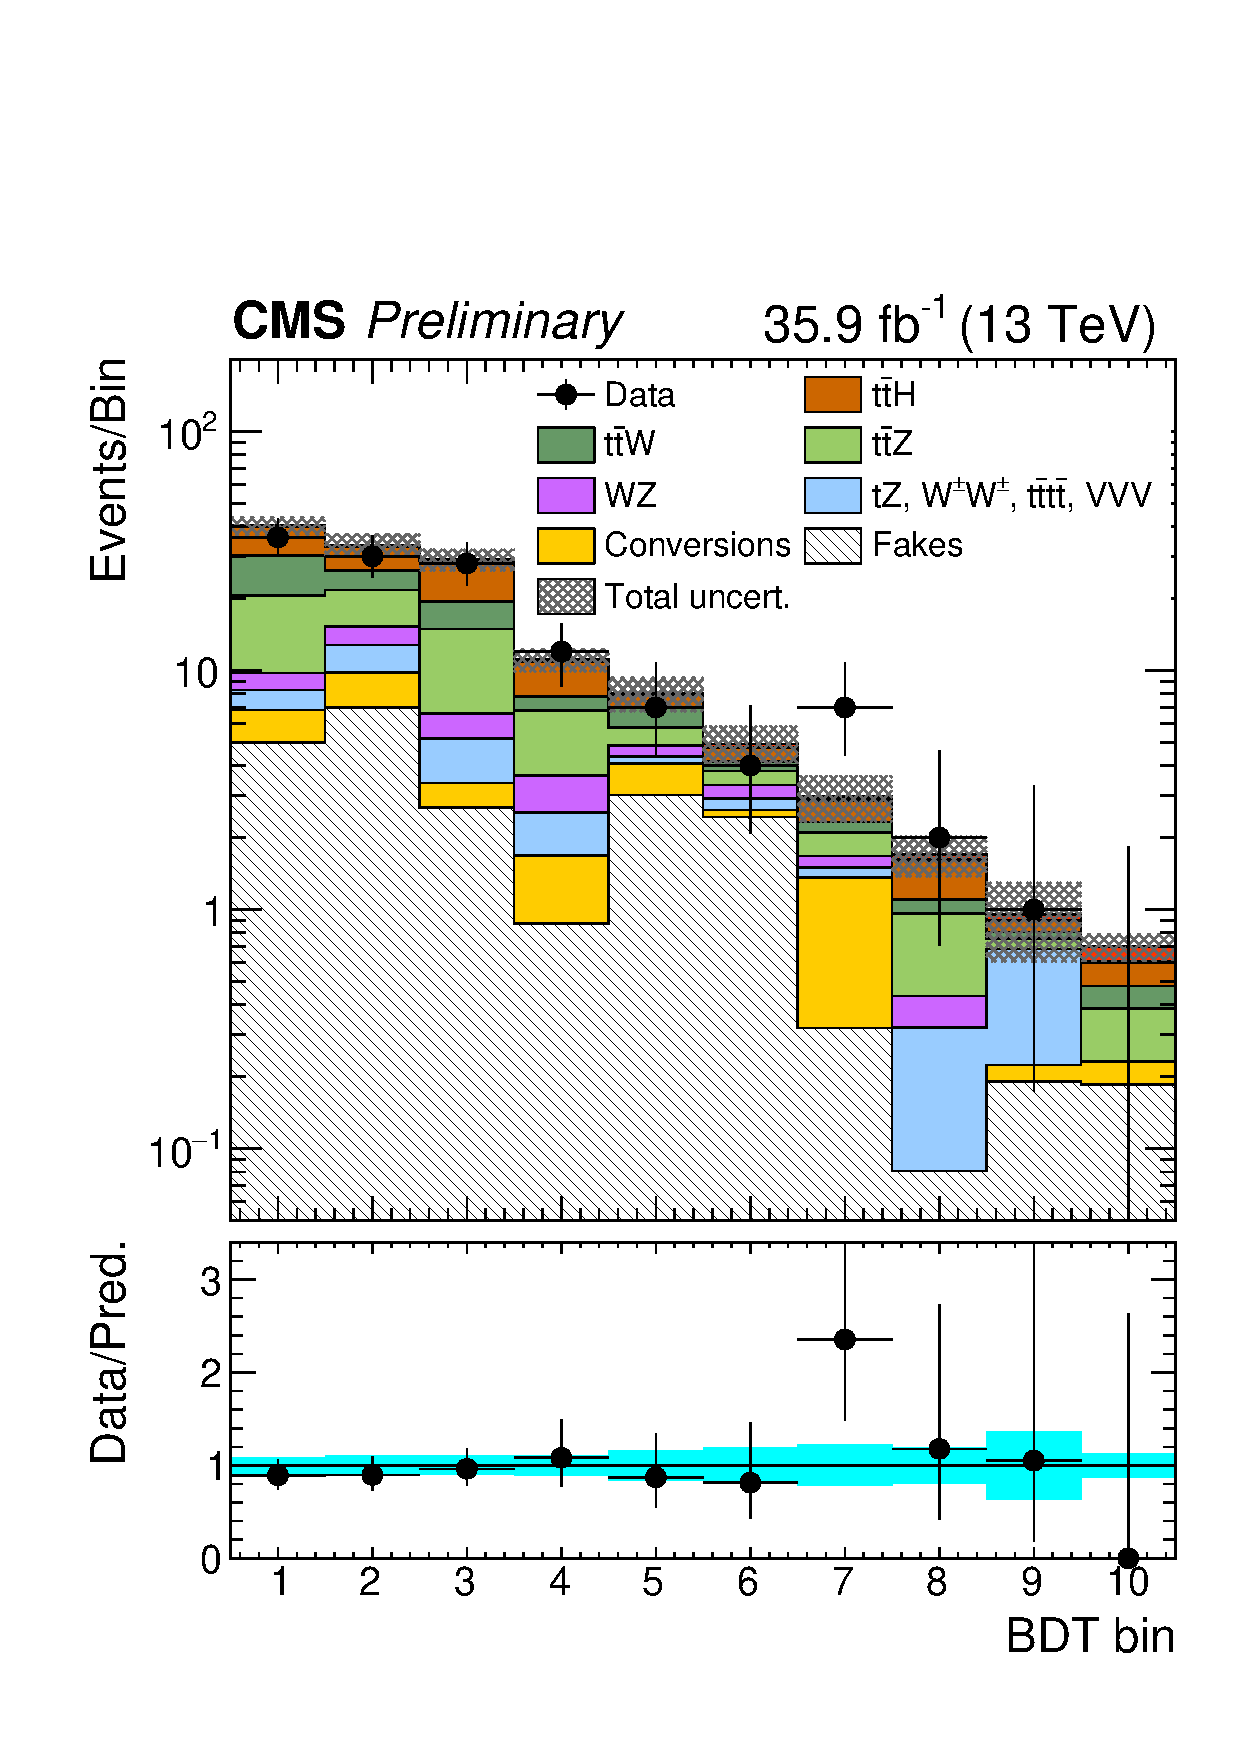
\includegraphics[width=0.32\textwidth]{Figures/postfit/tHq_3l_13TeV_fit_s_log.pdf}
    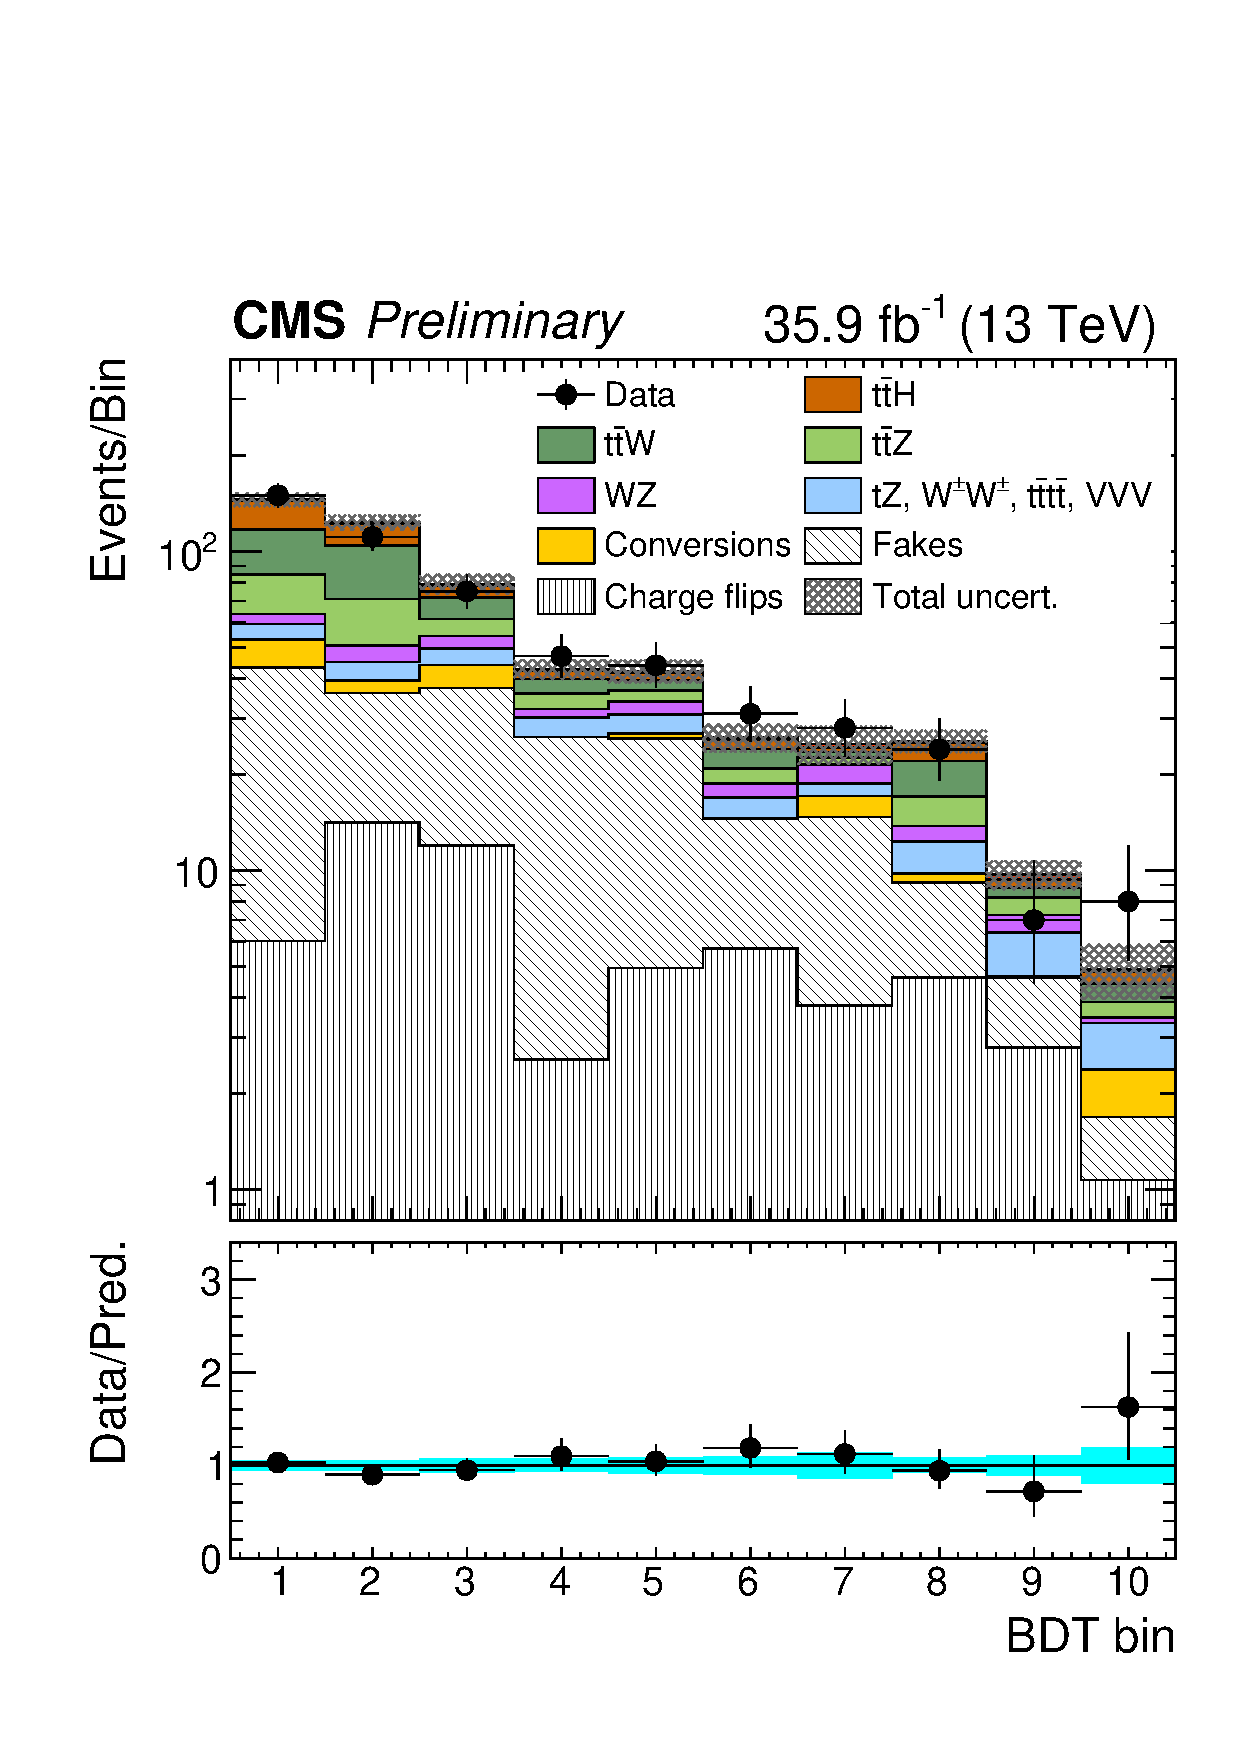
\includegraphics[width=0.32\textwidth]{Figures/postfit/tHq_2lss_em_13TeV_fit_s_log.pdf} 
    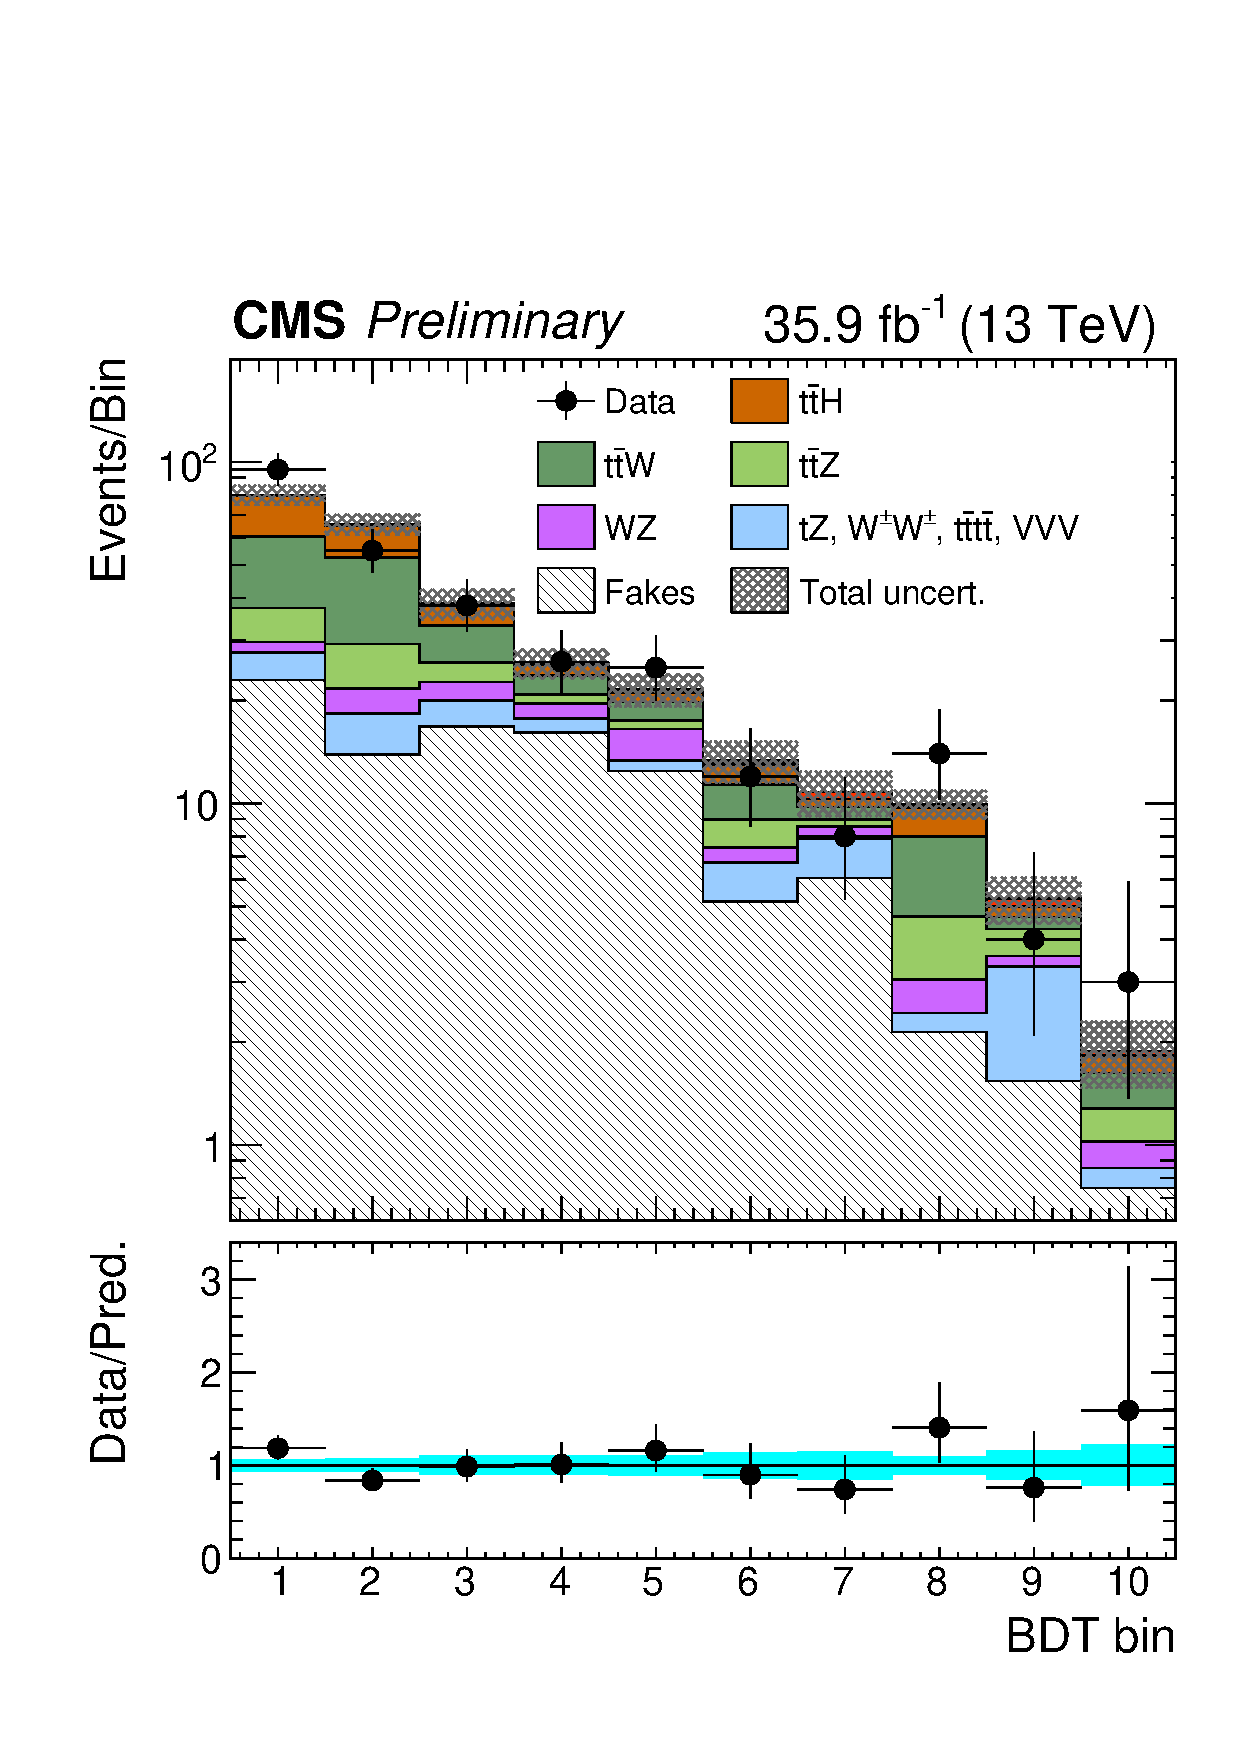
\includegraphics[width=0.32\textwidth]{Figures/postfit/tHq_2lss_mm_13TeV_fit_s_log.pdf}
  \end{center}
  \caption{Post-fit categorized BDT classifier outputs (on logarithmic scale) as used in the maximum likelihood fit for the three-lepton channel (left), \emu\ (center), and \mumu\ (right), for 35.9~\fbinv.
  In the box below each distribution, the ratio of the observed and predicted event yields is shown.
  \label{fig:aux_log_finalbins}}
\end{figure}

\begin{figure}[!h]
  \centering
  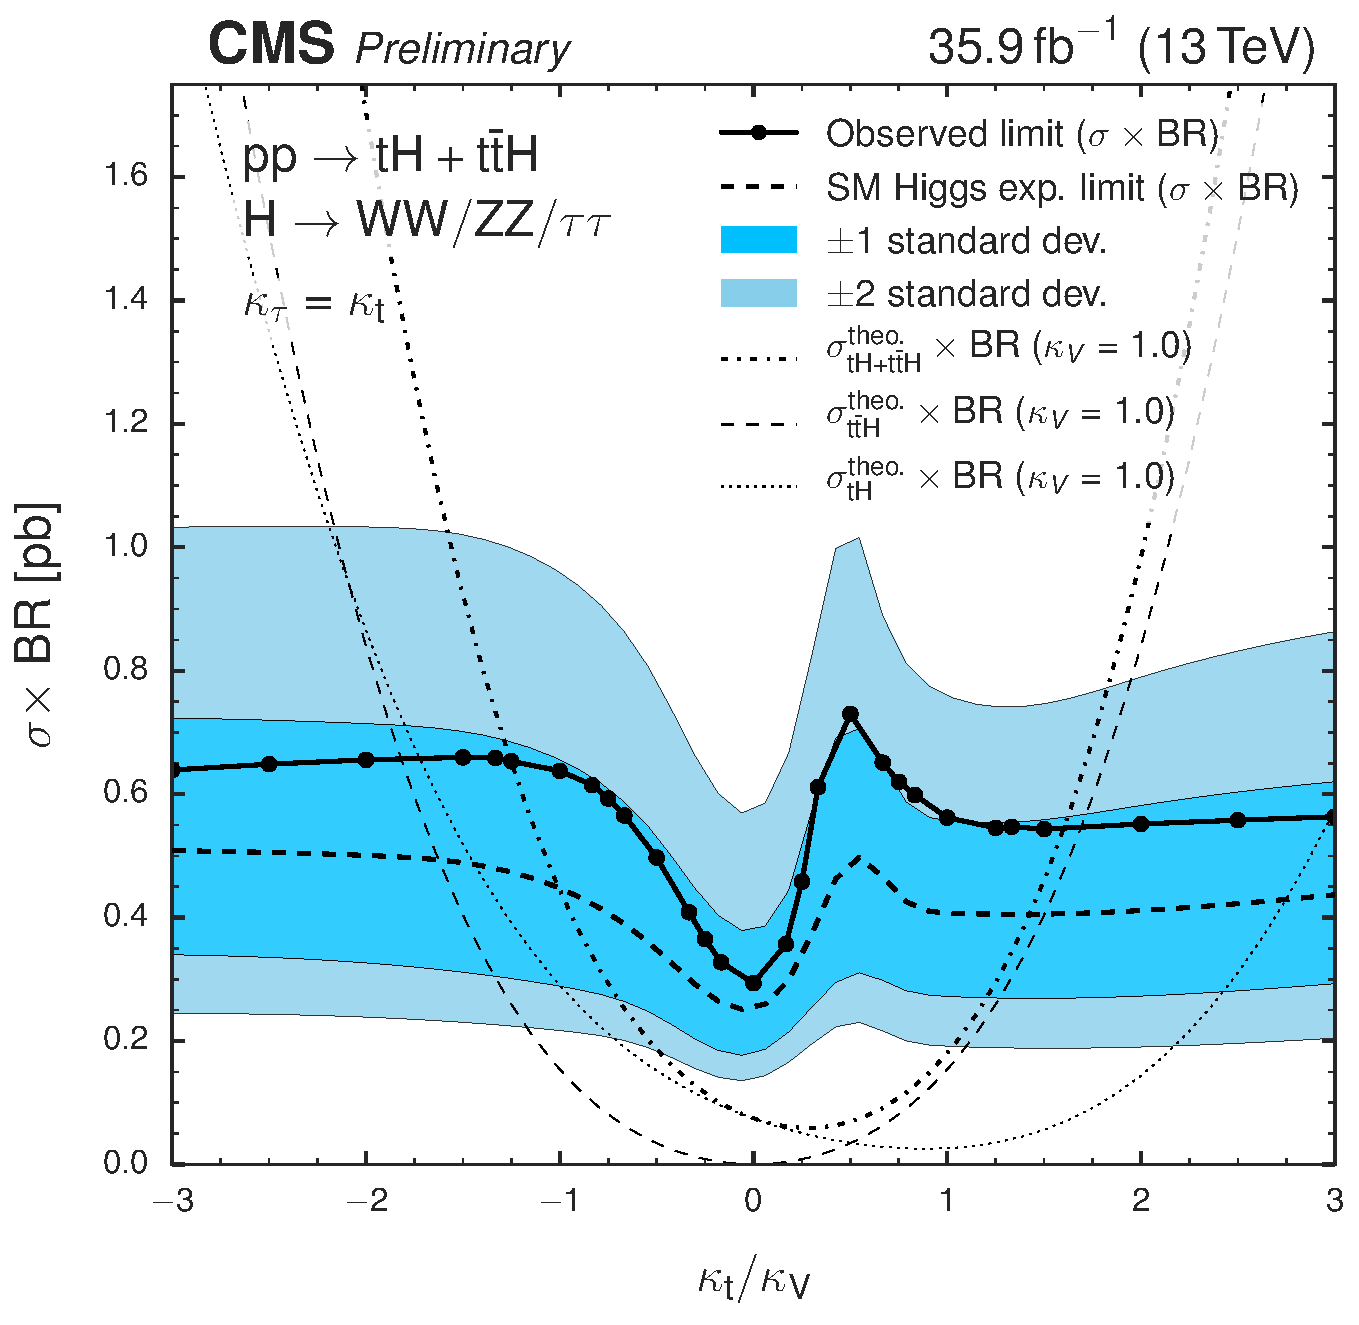
\includegraphics[width=0.8\textwidth]{Figures/xs_limits_K6_smexp.pdf}
  \caption{Observed and expected 95\% C.L. upper limit on the $\tH+\ttH$ cross section times $\PH\to\W\W^*+\tautau+\Z\Z^*$ branching fraction for different values of the coupling ratio \Ct/\CV. The expected limit is derived from a MC dataset of SM processes including the contributions from \ttH\ and \tH\ expected in the SM. %, and shown with its $\pm1\sigma$~(darker blue) and $\pm2\sigma$~(light blue) probability bands.
  \label{fig:aux_smexp_limits}}
\end{figure}




\clearpage
\bibliography{auto_generated}   % will be created by the tdr script.

%%%%%%%%%%%%%%%
\end{document}


